\section{Ergebnisse}
\label{Ergebnisse}
In diesem Kapitel werden die Ergebnisse der Implementierung vorgestellt. Zunächst werden die zentralen Funktionalitäten der Gruppenfunktion und HID vorgestellt. Daraufhin die Ergebnisse diskutiert und im Abschluss der Stand der Produktentwicklung vorgestellt.

\subsection{Evaluierung}


\subsubsection{Gruppenfunktion}
Bei der Gruppenfunktion war die größte Herausforderung der Implementierung, dass gerade in den HID Modi die Reihenfolge der Gruppe eingehalten werden muss damit die Messergebnisse in der Ausgabe wieder einem Werkzeug zuordbar sind. In Abbildung 7 ist die Ausgabe der Gruppenfunktion über den virtuelle COM-Port im Modus CDC zu sehen. Die Ausgabe wurde in Terminalprogramm RealTerm aufgefangen und die einzelnen Ausgaben der Gruppenfunktion durch rote Striche getrennt. Durch Betätigen des Fußtasters werden also jeweils die drei Zeilen zwischen den roten Strichen ausgegeben. Durch die Kanalnummern, die nur in diesem Modus Verwendung finden und jeweils am Anfang der Zeilen stehen, sind die Messergebnisse den einzelnen Geräten zuordbar. Zusätzlich wurden die Messuhren auf Messwerte eingestellt, die zu ihren Kanalnummern und Gruppennummern korrespondieren. 
\begin{figure}[H] 
	\centering
	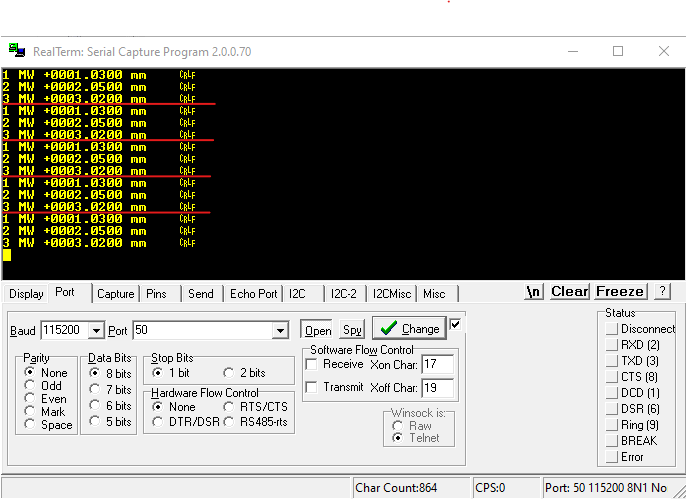
\includegraphics[width=\textwidth]{figures/GroupFeature.png}
	\caption{Durchführung von Messungen mit der Gruppenfunktion über CDC}
\end{figure}

Die gleichen Messungen sind in Abbildung 8 im Modus USB-HID durchgeführt. Durch Betätigung des Fußtasters wird jeweils eine Zeile Messwerte ausgegeben. Es ist ersichtlich, dass bei einer Vertauschung der Messergebnisse, bei echten Messdaten die von Zeile zu Zeile jeweils unterschiedlich sind, dies nicht nachvollzogen werden kann. Da hier jedoch die Einhaltung der Reihenfolge gezeigt werden soll, sind die Messergebnisse immer die Gleichen und korrespondieren zu ihren Gruppennummern. Es wird deutlich, dass auch bei mehreren durchgeführten Gruppenmessungen die Reihenfolge der Gruppe eingehalten wird.
\begin{figure}[H] 
	\centering
	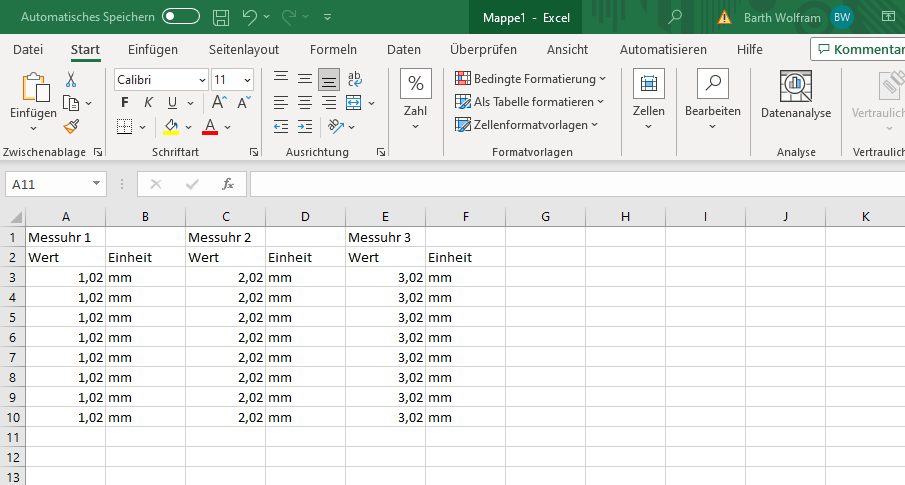
\includegraphics[width=\textwidth]{figures/USBHIDGroup.png}
	\caption{Durchführung von Messungen mit der Gruppenfunktion über HID}
\end{figure}

\subsubsection{Zeitmessungen HID}
Für die Modi USB-HID und BLE-HID ist die Zeit die verstreicht bis das gesamte Messergebnis eingetippt wurde das wichtigeste Gütekriterium der Implementierung neben der offentsichtlichen Fehlerfreiheit. In Abbildung 9 sind daher die Logausgaben der Aufrufe zur Funktion, die die einzelnen Tastendrücke an die USB-HID-Library übergibt zu sehen. In Klammern ist die verstrichene Zeit seit dem ersten Tastendruck in Millisekunden zu sehen. Abgesehen von der Zeitspanne zwischen dem ersten Tastendruck und Tasten loslassen, in der weniger als eine Millisekunde vergangen ist, liegen zwischen jedem einzelnen Aufruf genau zwei Millisekunden. Es ist zu vermuten, dass die Zeitspanne zwischen den ersten beiden Aufrufen niedriger ist, da die Daten noch nicht über USB gesendet wurden, sondern zwischengespeichert sind. Sobald begonnen wird die Daten tatsächlich über USB zu senden, vergehen zwischen zwei Tastendrücken genau zwei Millisekunden. Das Messergebniss wird schnell und gleichmäßig über USB eingetippt. Zu den Zeitstempeln 22 und 24 wird dabei die Tabulatortaste gedrückt um in einer Tabelle in die nächste Spalte zu wechseln, während zum Zeitpunkt 34 und 36 die Zeile terminiert wird und in die nächste Zeile gesprungen wird.
\begin{figure}[H] 
	\centering
	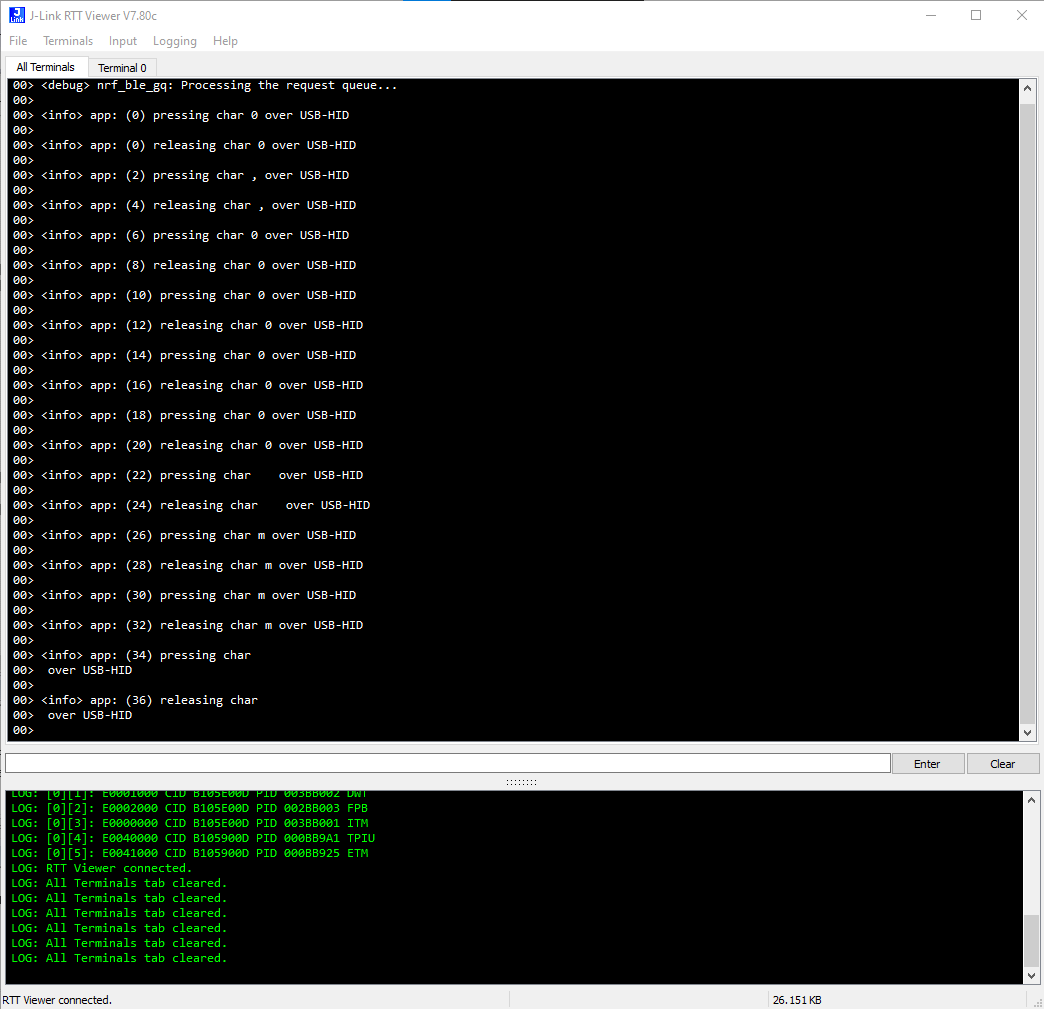
\includegraphics[width=\textwidth]{figures/USBHID.png}
	\caption{Logging einer Ausgabe eines Messergebnis über USB-HID}
\end{figure}

Anders ist das zeitliche verhalten bei Eingabe des Messergebnis über BLE-HID. In Abbildung 10 ist der Mitschnitt der BLE-Nachrichten des Fußschalters an den Computer bei einer verbundenen Messuhr zu sehen. Es wurde der Ellisys Bluetooth Analyzer verwendet. Hier ist auch zu sehen wie zum Zeitpunkt 13:30:35.883 das Messergebnis als HCT-Nachricht von der Messuhr an den Fußschalter übertragen wird. Ab dem Zeitpunkt 13:35.948 werden die Tastendrücke vom Fußschalter an den Computer übertragen. Dabei werden die Codes für Tastaturtasten übertragen und nicht die Codes der ASCII-Zeichen. Der Code 0 steht dabei für das loslassen einer Taste. Es wird deutlich, dass die einzelnen Tastendrücke mit unregelmäßigen Abständen eingetippt werden. Die Telegrame zwischen denen weniger als eine Millisekunde verstreicht werden dabei in einem Zeitslot übertragen. Es kommt in unregelmäßigen Zeitabständen dazu, dass mit ungefähr 110 Millisekunden eine verhältnismäßig lange Zeitspannen zwischen den einzelnen Nachrichten verstreicht, vorallem da das Connection Interval hier 30 Millisekunden beträgt und somit der Fußschalter deutlich mehr Zeitslots für weitere Übertragungen zur Verfügung hätte. Es wird beobachtet, dass die Ausgabe stottert.
\begin{figure}[H] 
	\centering
	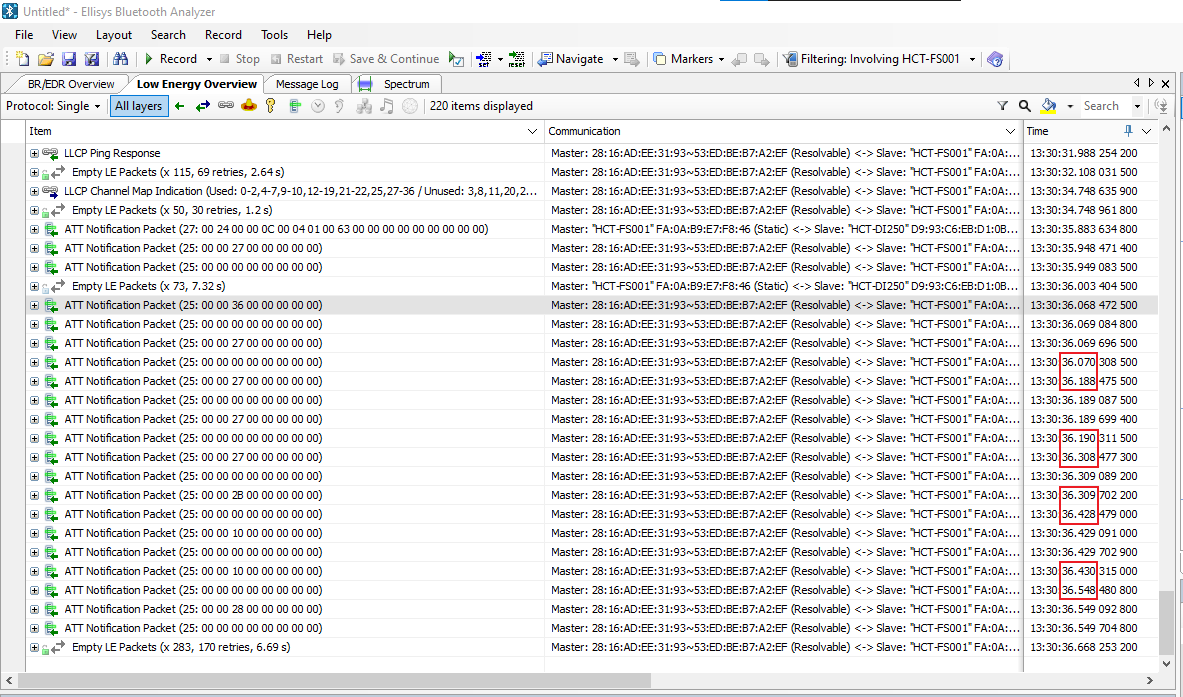
\includegraphics[width=\textwidth]{figures/BLEHID1device.png}
	\caption{Mitschnitt der BLE Nachrichten eines BLE-HID Messergebnis von einer verbundenen Messuhr}
\end{figure}

Dieses Verhalten verschärft sich, wenn mehrere Messuhren verbunden sind. In Abbildung 11 ist der Mitschnitt der BLE-Nachrichten der Tastendrücke bei drei verbundenen Messuhren zu sehen. Die Übertragungen treten wieder gehäuft auf. In einem Zeitslot werden mehrere Zeichen übertragen zwischen denen weniger als eine Millisekunde verstreicht, während die Zeit bis nur nächsten Übertragung mit 236 Millisekunden fast achtmal so groß wie das Connection Interval von 30 Millisekunden ist. Interessanterweise beträgt die Zeitdauer in allen der drei roten Kästen jeweils exakt 236 Millisekunden.
\begin{figure}[H] 
	\centering
	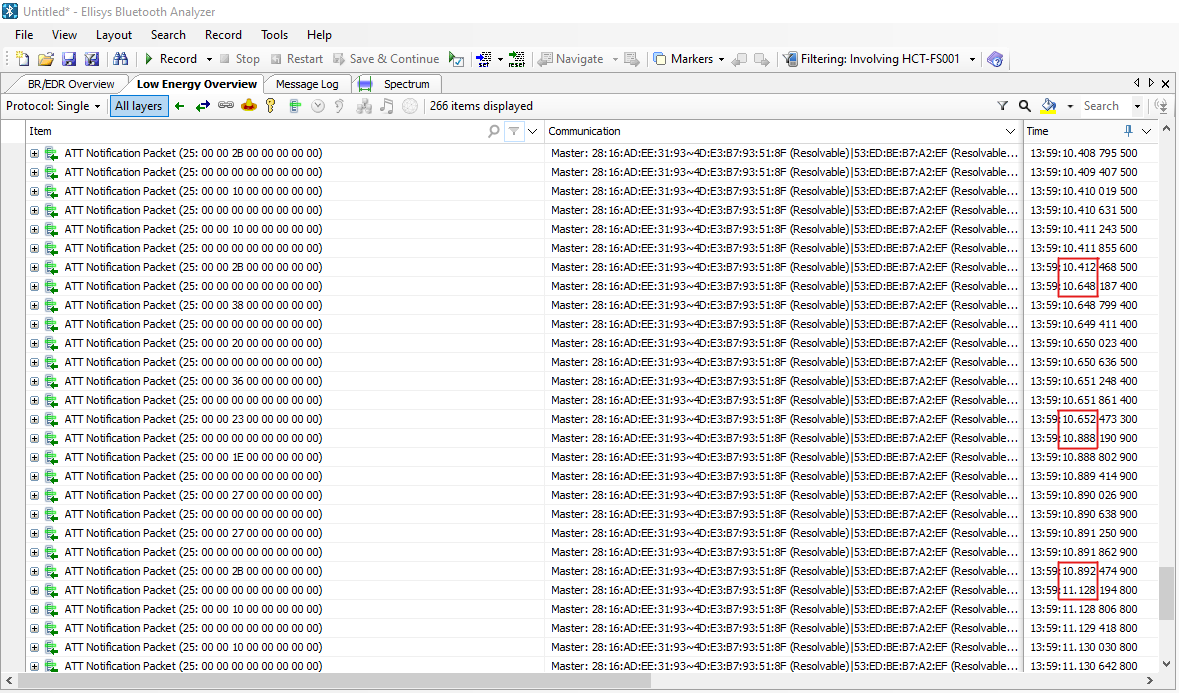
\includegraphics[width=\textwidth]{figures/BLEHID2device.png}
	\caption{Mitschnitt der BLE Nachrichten der BLE-HID Messergebnisse von drei verbundenen Messuhr}
\end{figure}

\subsection{Diskussion}
Die Koordinierung von mehreren Messuhren mit der Gruppenfunktion, sowie die Modi \ac{USB}-\ac{HID} und \ac{CDC} funktionieren fehlerfrei und werden als vollständig implementiert betrachtet. In Verbindung mit den HID Modi ist die Gruppenfunktion eine Funktionalität die es noch in keinem anderen Produkt gibt und ist damit eines der zentralen Verkaufsargumente. Bislang müssen Messuhren einzelnen entweder als HID-Device oder über die HCT-Windows-App, welche jedoch keine HID Funktionalität zur Verfügung stellt, verbunden werden.\\
Im Modus \ac{BLE}-\ac{HID} kommt es dazu, dass die Ausgabe stottert also in unregelmäßigen Abständen verhältnismäßig große Zeitspannen verstreichen bis die Ausgabe fortgeführt wird. Dabei steht in Verdacht, dass die Connection Intervalle bei mehreren bestehenden Verbindungen nicht gut koordiniert werden. In Abbildung 12

\begin{figure}[H] 
	\centering
	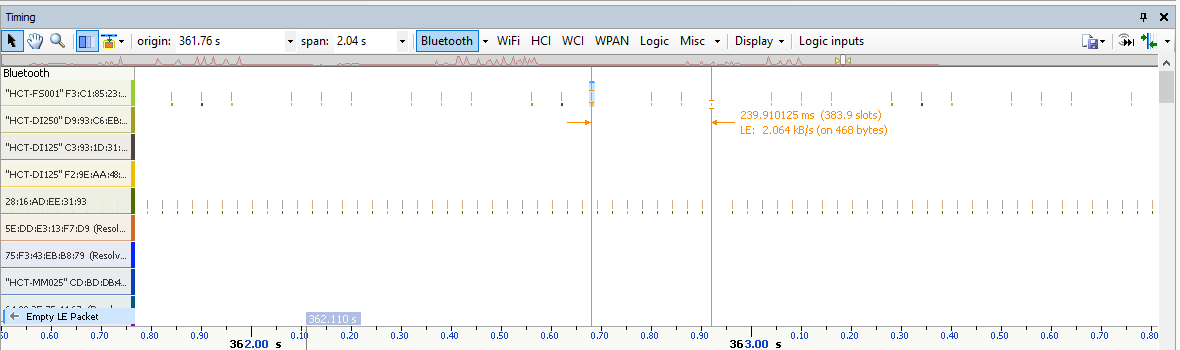
\includegraphics[width=\textwidth]{figures/ConnectionIntervalle.png}
	\caption{Diagramm der Connection Intervalle bei drei Messuhren und einer Verbindung zum Computer}
\end{figure}


\subsection{Stand Produktentwicklung}
Der Fußschalter und der Dongle sollen als eigenständige Produkte in das Sortiment der Hoffmann Group übernommen werden. Für sie werden jeweils Projekte vom Produktmanagement eröffnet. Dabei werden die Hardwareänderungen wie in Kapitel 5.4.1 beschrieben, in das Layout der Platine übernommen. Zusätzlich sollen die Pins, die den Chip in den Bootloader Mode versetzt, durch eine Taste von außen erreichbar gemacht werden. Außerdem sollen auch die SWE-Pads, die das Debugging auf dem Chip ermöglichen, erreichbar gemacht werden. Derzeitig sind sie auf der Seite mit der der Dongle auf die Platine gelötet wurde, weswegen sie nur sehr schwer abgreifbar sind. Die Prototypen dieser neuen Hardwareversion wurden gegen Ende dieser Arbeit erhalten und es wurde bereits festgestellt, dass die Taste die den Fußschalter in den Bootloadermodus versetzt nicht wie spezifiert funktioniert. Der Zulieferer der Platine muss diese daher erneut überarbeiten. Des weiteren werden umfassende Funk- und Reichweitenmessungen durchgeführt, da die ursprüngliche Platine dort nicht die Anforderungen erfüllte.\\
Der Modus \ac{BLE}-Windows-App wurde auf eine spätere Version verschoben, da die Integration der Messuhren und Messschieber in die Windows App andauert, sowie neue Geräte auf den Markt kommen sollen und deren Integration priorisiert wird. Eine Integration des Fußschalters ist daher noch nicht absehbar. Daher wurde die Implementierung des Modus zugunsten anderer Features bis auf Weiteres verschoben.\\
Insbesonders der Dongle ist bereits zu ersten Testläufen an ausgewählte Kunden gegeben worden und hat sich dort bereits bewährt. Desweiteren werden Codereviews mit anderen Entwicklern der Hoffmann Group durchgeführt.\\
Für die Funktionalität des Fußschalter beziehungsweise des Dongles wird eine Erfindungsmeldung herausgegeben und der Prozess der Patentierung der Technik wurde angestoßen. Siehe Anhang \ref{appendix:Erfindungsmeldung}.
